\documentclass{anstrans}
%%%%%%%%%%%%%%%%%%%%%%%%%%%%%%%%%%%
\title{Boundary Conditions for Diffusion in Flatland Geometry}
\author{Seth R.~Johnson \and Edward W.~Larsen}

%% uncomment these next five only if using anstrans
\institute{Department of Nuclear Engineering \& Radiological Sciences, University of Michigan, Ann Arbor, MI, 48109}
\email{sethrj@umich.edu \and edlarsen@umich.edu}
\usepackage{amssymb}
\usepackage{microtype}
\usepackage{graphicx}
\usepackage{booktabs} % \toprule, \midrule, \bottomrule
%%% INCLUDE FILE FOR DEFINITIONS
%%% These may require various packages.

% Shortcuts in regular text
\newcommand{\degs}{\ensuremath{^\circ}}
\newcommand{\EE}[1]{\ensuremath{\times 10^{#1}}}
\newcommand{\ttimes}{\ensuremath{{}\times{}}}
\newcommand{\cclicense}{%
  \smash{\raisebox{-0.45ex}{%
  \setlength{\unitlength}{1em}%
  \begin{picture}(1,1)%
    \put(0.5,0.5){\circle{1}}
    \put(0.5,0.5){\hbox to 0pt{\hss\raisebox{-.45ex}{\tiny\textsf{CC}}\hss}}
  \end{picture}%
  }}%
  \hskip -1em%
  \href{http://creativecommons.org/licenses/by-nc-sa/3.0/}%
  {\ \hskip 1em \textsf{BY-NC-SA}}%
}

%\newcommand{\horizsep}{{\par\noindent\centering\rule[.25ex]{.75\columnwidth}{2pt}\par}}
\newcommand{\horizsep}{\vspace{\baselineskip}\noindent\hspace{\stretch{1}}$
\ast\qquad \ast\qquad \ast\qquad
$ \hspace{\stretch{1}} \vspace{\baselineskip}}
\newcommand{\pytrt}{\textsf{PyTRT}}

% Research
\newcommand{\lop}[1]{\mathcal{L}\!\left[#1\right]}
\newcommand{\lopinv}[2]{\mathcal{I}_{#1}\!\left[#2\right]}
\newcommand{\Dtens}{\mat{D}}
\newcommand{\Etens}{\mat{E}}
\newcommand{\Identitytens}{\mat{I}}
\newcommand{\APone}{AP$_1$}
\newcommand{\Pone}{P$_1$}
\newcommand{\SN}{S$_N$}%{S$_\text{N}$}%{$S_N$}%
\newcommand{\PN}{P$_N$}%{P$_\text{N}$}%{$P_N$}%
\newcommand{\CN}{Crank--Nicolson} %Yes, it's Nic not Nich
\newcommand{\Eddington}{\mathcal{E}} %whatever symbol I decided for Eddington
\newcommand{\RadEn}{E} %whatever symbol I decide for radiation energy
\newcommand{\Sigmatr}{\Sigma_{\mathit{tr}}}

% Program names
\newcommand{\cpp}{\textsf{C\raisebox{0.2ex}{++}}}

% General math shortcuts
\newcommand{\ud}{\mathop{}\!\mathrm{d}}
\newcommand{\pder}[2]{\frac{\partial #1}{\partial #2}}
\newcommand{\oder}[2]{\frac{\mathrm{d} #1}{\mathrm{d} #2}}
\newcommand{\tpder}[2]{{\partial #1}/{\partial #2}} %inlined
\newcommand{\toder}[2]{{\mathrm{d} #1}/{\mathrm{d} #2}} %inlined
\newcommand{\lra}{ \quad \Longrightarrow \quad }
\newcommand{\eexp}{\mathop{}\!\mathrm{e}} % upright ``e'' for exponent
\newcommand{\expp}[1]{\exp\!\left( {#1} \right)} % exp with parentheses
\newcommand{\qeq}{\stackrel{\mathrm{?}}{=}}

% Probability
\newcommand{\expectation}[1]{\mathop{}\!\mathrm{E}\!\left[ #1 \right]}
\DeclareMathOperator{\Var}{Var} % variance

% Asymptotic analysis
\DeclareMathOperator{\Ei}{Ei} % Exponential function
\newcommand{\lapl}[1]{\mathcal{L}[{#1}]} %laplace

%change the Re and Im operators from fancy curly letters
\DeclareMathOperator{\MathOpRe}{Re}
\renewcommand{\Re}{\MathOpRe}
\DeclareMathOperator{\MathOpIm}{Im}
\renewcommand{\Im}{\MathOpIm}

%imaginary ``i'' , upright 'i' or \imath
\newcommand{\iimag}{\mathrm{i}}

% Finite differences
\newcommand{\hot}{\text{h.o.t.}}
\newcommand{\inv}{^{-1}}

% Numerical Linear Algebra
\newcommand{\conj}{^{\ast}} % complex conjugate (transpose)
\newcommand{\norm}[1]{\left\| #1 \right\|} % double pipe
\newcommand{\abs}[1]{\left| #1 \right|} % single pipe
\newcommand{\eps}{\varepsilon}
\DeclareMathOperator{\fl}{fl}

\DeclareMathOperator{\acosh}{arccosh} 

% Define a command to write a nice-looking element, e.g. 4,2 He
\newcommand{\elem}[3]{\ensuremath{{}^{{#1}}_{{#2}}\mathrm{{#3}}}}

% Vector definitions
\newcommand{\mat}[1]{\mathbf{#1}} %matrix is bold upright
\renewcommand{\vec}[1]{\bm{#1}} %vector is bold italic
\newcommand{\op}[1]{\mathsf{#1}} % ``operator'' is sans serif

\newcommand{\vd}{\bm{\cdot}} % slightly bold vector dot
\newcommand{\del}{\vec{\nabla}} % gradient (Del) is bold
\newcommand{\grad}{\vec{\nabla}} % gradient

%\newcommand{\abr}[1]{\langle {#1} \rangle}
\newcommand{\abr}[1]{\left\langle {#1} \right\rangle} % angle brackets for avg.

%% topbox is useful in extended definitions of math terms inside an align
\newcommand{\topbox}[2][0.6]{\parbox[t]{#1\columnwidth}{\raggedright{}#2}}

% commands to make text in math mode appear as zero-width (better-looking
% integrals/sums, e.g.)
% from mathmode.pdf page 74, or Alexander R. Perlis ``A complement to \smash,
% \llap, and \rlap''

\def\mathllap{\mathpalette\mathllapinternal}
	\def\mathllapinternal#1#2{%
	\llap{$\mathsurround=0pt#1{#2}$}%
}
\def\clap#1{\hbox to 0pt{\hss#1\hss}}%
\def\mathclap{\mathpalette\mathclapinternal}%
\def\mathclapinternal#1#2{%
	\clap{$\mathsurround=0pt#1{#2}$}%
}
\def\mathrlap{\mathpalette\mathrlapinternal}%
\def\mathrlapinternal#1#2{%
	\rlap{$\mathsurround=0pt#1{#2}$}%
}


% graphics paths
\graphicspath{{/Users/seth/_research/figures/}}
\makeatletter
\def\input@path{{/Users/seth/_research/figures/}}
\makeatother

\renewcommand{\bottomfraction}{0.99}
\renewcommand{\topfraction}{0.99}

%\usepackage{setspace}
%\doublespacing

\date{2011/05/30}
%%%%%%%%%%%%%%%%%%%%%%%%%%%%%%%%%%%
\begin{document}
%%%%%%%%%%%%%%%%%%%%%%%%%%%%%%%%%%%%%%%%%%%%%%%%%%%%%%%%%%%%%%%%%%%%%%%%%%%%%%%%
\section{Introduction}
Flatland geometry, a fictional two-dimensional space where particles are
constrained to the page, has recently proven useful in
transport methods development \cite{Asa2008,Lar2009c}. Because the flatland phase
space is $(x,y,\theta)$ rather than the two-dimensional $(x,y,\mu,\theta)$,
flatland
is a computationally less burdensome testing ground that still retains the
complexity of multidimensional geometry.

Previous work in flatland has shown that the diffusion
coefficient for flatland geometry $\frac{1}{2\sigma}$ is different from
the physical diffusion coefficients $\frac{1}{3\sigma}$, but the correct
formulation for flatland diffusion boundary conditions has remained an
unanswered and indeed unasked question.

This summary derives both a Marshak boundary condition and a variational
boundary condition for diffusion in flatland. An accurate diffusion boundary
condition is imperative for anyone looking to benchmark a new method in
flatland against a diffusion solution.

%%%%%%%%%%%%%%%%%%%%%%%%%%%%%%%%%%%%%%%%%%%%%%%%%%%%%%%%%%%%%%%%%%%%%%%%%%%%%%%%
\section{Analysis}
The steady-state, monoenergetic transport equation is
\begin{equation}\label{eq:generalTransport}
  \vec{\Omega}\vd \grad \psi + \sigma \psi
  = \frac{c \sigma}{\omega_0} \int_{\Omega} \psi \ud\Omega + \frac{q}{\omega_0}
  \quad \vec{x}\in V,\ \vec{\Omega}\in \Omega \,,
\end{equation}
where $\vec{\Omega}$, $\Omega$, and $\omega_0$ depend on whether the geometry
is flatland or 2-D. We consider a specified incident boundary condition:
\begin{equation} \label{eq:ssBndy}
  \psi(\vec{x}, \vec{\Omega}) = \psi^b(\vec{x}, \vec{\Omega})\,,
  \quad \vec{x}\in \partial V,\ \vec{\Omega} \vd \vec{n} < 0\,.
\end{equation}

In 2-D geometry, $\vec{\Omega}=\sqrt{1-\mu^2} \cos \theta \vec{i} +
\sqrt{1-\mu^2} \sin \theta \vec{j}$; and in flatland, $\vec{\Omega}=\cos \theta
\vec{i} + \sin \theta \vec{j}$. The domain of angular integration $\Omega$ in
2-D is $-1\le\mu\le1$, $0 \le \theta < 2\pi$; in flatland, it is $0 \le \theta
< 2\pi$. These lead to the different angular moment identities
\begin{equation}\label{eq:omegaIdentities}
  \omega_m = \int_{\Omega} \abs{\vec{\Omega}\vd \vec{i}}^m \ud\Omega\,.
\end{equation}
In 2D, $\omega_0=4\pi$, $\omega_1=2\pi$, and $\omega_2=\frac{4\pi}{3}$.
However, in flatland, $\omega_0=2\pi$, $\omega_1=4$, and $\omega_2=\pi$. The
differences between those sets of identities lead to a different diffusion 
coefficient and different boundary conditions.

%The diffusion approximation begins by assuming that $\psi$ is linear in angle:
%\begin{equation*}
%  \psi(\vec{x}, \vec{\Omega}) \approx f(\vec{x}) + \vec{\Omega} \vd
%  \vec{g}(\vec{x})\,.
%\end{equation*}
%The zeroth angular moment of $\psi$ determines $f$:
%\begin{equation*}
%  \phi = \int_\Omega \psi \ud \Omega
%= \int_\Omega \left( f + \vec{\Omega}\vd \vec{g} \right) \ud\Omega
%= \int_\Omega\ud\Omega f + 0
%= \omega_0 f \,,
%\end{equation*}
%so $f = \phi/\omega_0$. Similarly, the first moment of $\psi$ gives $g$:
%\begin{equation*}
%  \vec{J} = \int_\Omega \vec{\Omega} \psi \ud \Omega
%= f \int_\Omega \vec{\Omega} \ud\Omega
%  + \vec{g} \vd \int_\Omega \vec{\Omega}\vec{\Omega} \ud\Omega
%= \omega_2 \vec{g} \,,
%\end{equation*}
%so $\vec{g} = \vec{J}/\omega_2$, which gives the \Pone\ approximation for
%$\psi$:
%\begin{equation}\label{eq:ssPone}
%  \psi(\vec{x}, \vec{\Omega})
%  \approx \frac{1}{\omega_0} \phi(\vec{x})
%  + \frac{1}{\omega_2} \vec{\Omega} \vd \vec{J}(\vec{x})
%\end{equation}
%
%The diffusion approximation is a closure for the first angular moment of
%the transport equation, so we now take the first moment of the transport
%equation and substitute
%Eq.~\eqref{eq:ssPone}:
%\begin{align*}
%  \grad \vd \int_\Omega \vec{\Omega} \vec{\Omega} \psi
%  \ud\Omega
%  + \sigma \int_\Omega \vec{\Omega} \psi \ud\Omega
%  &= \frac{1}{\omega_0} \phi(\vec{x}) \int_\Omega \vec{\Omega} \ud\Omega
%  \\
%  \grad \vd \int_\Omega \vec{\Omega} \vec{\Omega} \psi(\vec{x}, \vec{\Omega})
%  \ud\Omega
%  + \sigma \vec{J}
%  &= 0
%  \\
%  \grad \vd \int_\Omega \vec{\Omega} \vec{\Omega} \left(
%  \frac{1}{\omega_0}\phi + \frac{1}{\omega_2} \vec{\Omega} \vd \vec{J}
%  \right) \ud\Omega
%  + \sigma \vec{J}
%  &= 0
%  \\
%  \frac{\omega_2}{\omega_0} \grad \phi + \sigma \vec{J} &= 0 \,.
%\end{align*}
Under the assumption that $\psi$ is linear in angle, the first angular moment
of the transport equation can be reduced to Fick's law, expressed using the
identities of Eq.~\eqref{eq:omegaIdentities}:
\begin{equation} \label{eq:fickGeneral}
  \vec{J}(\vec{x})
  = - \frac{\omega_2}{\omega_0} \frac{1}{\sigma(\vec{x})} \grad \phi(\vec{x})
  \equiv -D(\vec{x}) \grad \phi(\vec{x})\,.
\end{equation}
In 2-D and 3-D, $\omega_2/\omega_0 = (4\pi / 3) / (4\pi) = 1/3$; however, in
flatland, $\omega_2/\omega_0 = \pi / (2\pi) = 1/2$. Thus, $D=\frac{1}{3\sigma}$ in
2-D but $D=\frac{1}{2\sigma}$ in flatland.

Fick's law and the linear-in-angle approximation give the diffusion
approximation to the angular flux:
\begin{equation} \label{eq:diffusionIntensity}
  \psi(\vec{x}, \vec{\Omega})
  = \frac{1}{\omega_0} \left[ \phi(\vec{x})
  - \frac{1}{\sigma(\vec{x})}
  \vec{\Omega} \vd \grad \phi(\vec{x}) \right] \,.
\end{equation}

%%%%%%%%%%%%%%%%%%%%%%%%%%%%%%%%%%%%%%%%%%%%%%%%%%%%%%%%%%%%%%%%%%%%%%%%%%%%%%%%
\subsection{Marshak Boundary Condition}
The Marshak boundary condition preserves the incident
current on the boundary. It is derived by substituting the approximate diffusion
angular flux from Eq.~\eqref{eq:diffusionIntensity} into the boundary condition,
Eq.~\eqref{eq:ssBndy}, multiplying by $\abs{\vec{\Omega}\vd \vec{n}}$, and integrating over
incident directions:
\begin{align*}
\int_{\vec{\Omega}\vd \vec{n} < 0 } \abs{\vec{\Omega}\vd \vec{n}}
\psi^b \ud\Omega
 &= 
\int_{\vec{\Omega}\vd \vec{n} < 0 } \abs{\vec{\Omega}\vd \vec{n}} 
 \frac{1}{\omega_0} \left[ \phi - \frac{1}{\sigma}
  \vec{\Omega} \vd \grad \phi \right]
  \ud\Omega
\end{align*}
After some algebra, using the identities in Eq.~\eqref{eq:omegaIdentities}, we
find an expression for the Marshak boundary condition for general geometries:
\begin{equation} \label{eq:marshak}
\frac{2\omega_0}{\omega_1}
\int_{\vec{\Omega}\vd \vec{n} < 0 } \abs{\vec{\Omega}\vd \vec{n}}
\psi^b \ud\Omega
=
\phi + \frac{\omega_2}{\omega_1}\frac{1}{\sigma} \vec{n} \vd \grad \phi \,.
\end{equation}
In 2D, this evaluates to the standard Marshak boundary condition with
extrapolation distance $\frac{\omega_2}{\omega_1} = \frac23$, but in flatland
it gives
\begin{equation*}
\pi J^{-} = \phi + \frac{\pi}{4}\frac{1}{\sigma} \vec{n} \vd \grad \phi
= \phi + \frac{\pi}{2} D \vec{n} \vd \grad \phi\,.
\end{equation*}
Thus, the flatland extrapolation distance of $\frac{\pi}{4} \approx 0.7854$
is about 18\% longer than in 2D.
Physically, this has the interpretation that in 2D, a significant fraction of
particles are traveling at a steep angle to the $x$-$y$ plane, yielding a
shorter extrapolation distance, i.e.~a steeper slope for $\phi$ on the boundary.

%%%%%%%%%%%%%%%%%%%%%%%%%%%%%%%%%%%%%%%%%%%%%%%%%%%%%%%%%%%%%%%%%%%%%%%%%%%%%%%%
\subsection{Variational Boundary Condition}
It is well known that the Marshak boundary condition is \emph{ad hoc}, and that
the correct boundary condition for diffusion is derived from an
asymptotic matched boundary layer analysis \cite{Mal1991}. A reasonably simple
method of deriving a more accurate boundary condition is to use a variational analysis.

We consider a steady-state, homogeneous, purely scattering transport problem in
a semi-infinite plane, $-\infty < x < \infty$, $0 < y < \infty$,
\begin{subequations} \label{eqs:flatTransport}
\begin{equation}\label{eq:flatTransportVol}
  \vec{\Omega}\vd \grad \psi + \sigma \psi
  = \frac{\sigma}{2\pi} \int_{0}^{2\pi} \psi \ud\theta\,, \quad 0 \le \theta <
  2\pi\,.
\end{equation}
It has a uniform incident boundary condition,
\begin{equation}\label{eq:flatTransportBndy}
  \psi(x, 0, \theta) = \psi^b(\theta)\,,
  \quad 0 \le \theta < \pi \,.
\end{equation}
\end{subequations}
Also, because there is no variation in the boundary condition or $\sigma$ along
the $x$ axis, $\tpder{\psi}{x}=0$, and Eq.~\eqref{eq:flatTransportVol} becomes
the one-dimensional transport equation 
\begin{equation}\label{eq:flatMarshak}
  \sin \theta \pder{}{y}\psi(y,\theta) + \sigma \psi(y,\theta)
  = \frac{\sigma}{2\pi} \int_{0}^{2\pi} \psi(y,\theta') \ud \theta'\,.
\end{equation}
This is \emph{not} the same one-dimensional transport equation as in slab
geometry.
We define the $y$ components of the angular moments of $\psi$ as
\begin{equation} \label{eq:flatPhi}
  \phi_m(y) = \int_{0}^{2\pi} (\vec{\Omega}\vd\vec{j})^m \psi(y,\theta) \ud\theta
  = \int_{0}^{2\pi} (\sin\theta)^m \psi(y,\theta) \ud\theta \,.
\end{equation}

As $y\to\infty$, the angular flux $\psi$ will approach a constant $\varphi/2\pi$,
which gives $\phi_0(\infty)=\varphi$. Concordantly, $\phi_1(\infty)=0$.

Operating on the transport equation with $\int_{0}^{2\pi} (\sin\theta)^m (\cdot)
\ud\theta$ gives the $m$th angular moment in the $y$ direction:
\begin{align}
 % \nonumber
 % \pder{}{y} \int_{0}^{2\pi} (\sin\theta)^{m+1} \psi \ud\theta
 % + \sigma \int_{0}^{2\pi} (\sin\theta)^{m} \psi \ud\theta
 % &= \frac{\sigma}{2\pi} \int_{0}^{2\pi} \psi \ud \theta'
 % \int_{0}^{2\pi} (\sin\theta)^{m} \ud\theta
 % \\
  \label{eq:flatMoments}
  \pder{\phi_{m+1}}{y}
  + \sigma \phi_{m}
  &= \frac{\sigma}{2\pi} \phi_{0}
  \int_{0}^{2\pi} (\sin\theta)^{m} \ud\theta\,.
\end{align}
For $m=0$, the conservation equation, Eq.~\eqref{eq:flatMoments} evaluates to
\begin{equation*}
  \pder{\phi_{1}}{y}
  + \sigma \phi_{0}
  = \frac{\sigma}{2\pi} \phi_{0} (2\pi)
  \lra
  \pder{\phi_{1}}{y} = 0\,.
\end{equation*}
That means the current is a constant, and because $\phi_1(\infty)=0$,
that constant is zero.

Evaluating Eq.~\eqref{eq:flatMoments} for $m=1$ and using the result that
$\phi_{1}=0$, we find
\begin{equation*}
  \pder{\phi_{2}}{y}
  + \sigma \phi_{1}
  = \frac{\sigma}{2\pi} \phi_{0} (0)
  \lra
  \pder{\phi_{2}}{y} = 0\,.
\end{equation*}
Thus $\phi_{2}$ is also a constant. As $y\to\infty$, $\psi\to\varphi/2\pi$, so
\begin{equation*}
  \phi_{2} = \int_{0}^{2\pi} (\sin\theta)^2 \frac{\varphi}{2\pi} \ud\theta
  = \frac{1}{2} \varphi\,.
\end{equation*}
% in 1D, this would be $\int_{-1}^{1}\mu^2\frac{\varphi}{2} \ud \mu =
% \frac{1}{3} \varphi$.

Now, since $\phi_1=0$, we can add $\alpha \phi_1$ to this equation for any
$\alpha$:
\begin{align*}
 %\alpha\phi_1 + \phi_{2} &= \frac{\varphi}{2} \\
 \int_{0}^{2\pi} (\alpha \sin\theta + \sin^2\theta)
 \psi(y,\theta) \ud\theta
 &= \frac{\varphi}{2}\,.
\end{align*}
At the boundary $y=0$, $\psi=\psi^b$ for incident angles $0 \le \theta < \pi$. The
variational analysis makes the reasonable approximation that, to leading order,
the exiting particles are isotropically distributed, $\psi(0,\theta)=\psi^\text{out}$.
\begin{equation*}
 \int_{0}^{\pi} (\alpha \sin\theta + \sin^2\theta)
 \psi^b(\theta) \ud\theta
 + \int_{\pi}^{2\pi} (\alpha \sin\theta + \sin^2\theta)\ud\theta \psi^\text{out}
 = \frac{\varphi}{2}\,.
\end{equation*}
The value $\alpha=\pi/4$ eliminates the integral over outgoing directions and
gives a relation between moments of the incident angular flux and the
magnitude of the angular flux as $y\to\infty$:
\begin{equation}\label{eq:varBoundary}
  \int_{0}^{\pi} \left( \frac{\pi}{4} \sin\theta + \sin^2\theta \right)
 \psi^b(\theta) \ud\theta
 = \frac{\varphi}{2}\,.
\end{equation}

We wish our boundary condition to preserve the value of $\varphi$ when the
diffusion method is used, so we substitute the diffusion approximation,
Eq.~\eqref{eq:diffusionIntensity}:
\begin{align*}
 \varphi &= 2\int_{0}^{\pi} \left( \frac{\pi}{4} \sin\theta + \sin^2\theta \right)
 \psi^b(\theta) \ud\theta
 \\
 &= 
  2\int_{0}^{\pi} \left( \frac{\pi}{4} \sin\theta + \sin^2\theta \right)
 \left( \frac{1}{2\pi} \phi -
  \frac{1}{\sigma} \sin\theta \pder{\phi_0}{y}\right)\ud\theta
\\
 &= 
  \phi
- \left( \frac{\pi}{8} + \frac{4}{3\pi} \right) \frac{1}{\sigma} \pder{\phi_0}{y}
\,.
\end{align*}
In this problem, we chose a boundary surface normal of $\vec{n}=-\vec{j}$. Now
replacing $\sin \theta$ with $-\vec{\Omega}\vd\vec{n}$, we get the 
variational boundary condition for flatland diffusion,
\begin{multline} \label{eq:flatVarBc}
\int_{\vec{\Omega}\vd\vec{n} < 0} \left[ \frac{\pi}{2}
\abs{\vec{\Omega}\vd\vec{n}} + 2 (\vec{\Omega}\vd\vec{n})^2 \right]
\psi^b(\vec{x}, \vec{\Omega}) \ud\Omega
\\
= 
  \phi(\vec{x})
  - \left( \frac{\pi}{8} + \frac{4}{3\pi} \right) \frac{1}{\sigma}
  \vec{n}\vd\grad \phi(\vec{x})\,.
\end{multline}
Compared to the flatland Marshak boundary condition,
Eq.~\eqref{eq:flatMarshak}, the variational boundary condition not only yields a
different extrapolation distance $\frac{\pi}{8} + \frac{4}{3\pi} \approx
0.8171$ but also uses a different moment of the incident boundary flux.

%%%%%%%%%%%%%%%%%%%%%%%%%%%%%%%%%%%%%%%%%%%%%%%%%%%%%%%%%%%%%%%%%%%%%%%%%%%%%%%%
\section{Numerical Results}
As a test problem, we consider a homogeneous flatland problem with a
total cross section $\sigma=1$ and scattering ratio $c=0.99$. It lives on the
domain $0 \le x \le 2$, $0 \le y \le 10$, with reflecting boundaries on the left,
right, and top sides. The bottom side has a specified boundary
condition with unit incident current, and we consider three different angular
distributions.

The first distribution is isotropic, $\psi^b(\theta) = \frac{1}{2}$. The second
is a normally incident flux, with all particles entering
perpendicular to the surface, $\psi^b(\theta) = \delta(\theta -
\frac{\pi}{2})$. The third incident distribution is at a grazing angle, with 
$\psi^b(\theta) = 10 \delta(\theta - \sin^{-1}.1)$.

Figure~\ref{fig:isotropic} shows a line-out of the scalar flux $\phi_0$ along
$x=1$ for an isotropic incident source. Because the left-hand sides of
Eqs.~\eqref{eq:flatMarshak} and~\eqref{eq:flatVarBc} are the same, the
differences in the solution are only due to the slightly different
extrapolation distance.

However, for the highly anisotropic normal and grazing cases,
Figs.~\ref{fig:delta} and~\ref{fig:grazing}, the Marshak boundary fails to
limit to the transport solution outside of the boundary layer. As
expected, the variational boundary condition does a much better job of
approximating the interior solution of the scalar flux.


\begin{figure}[htb!]
  \centering
  \hspace{-.5in}
  % GNUPLOT: LaTeX picture with Postscript
\begingroup
  \makeatletter
  \providecommand\color[2][]{%
    \GenericError{(gnuplot) \space\space\space\@spaces}{%
      Package color not loaded in conjunction with
      terminal option `colourtext'%
    }{See the gnuplot documentation for explanation.%
    }{Either use 'blacktext' in gnuplot or load the package
      color.sty in LaTeX.}%
    \renewcommand\color[2][]{}%
  }%
  \providecommand\includegraphics[2][]{%
    \GenericError{(gnuplot) \space\space\space\@spaces}{%
      Package graphicx or graphics not loaded%
    }{See the gnuplot documentation for explanation.%
    }{The gnuplot epslatex terminal needs graphicx.sty or graphics.sty.}%
    \renewcommand\includegraphics[2][]{}%
  }%
  \providecommand\rotatebox[2]{#2}%
  \@ifundefined{ifGPcolor}{%
    \newif\ifGPcolor
    \GPcolortrue
  }{}%
  \@ifundefined{ifGPblacktext}{%
    \newif\ifGPblacktext
    \GPblacktexttrue
  }{}%
  % define a \g@addto@macro without @ in the name:
  \let\gplgaddtomacro\g@addto@macro
  % define empty templates for all commands taking text:
  \gdef\gplbacktext{}%
  \gdef\gplfronttext{}%
  \makeatother
  \ifGPblacktext
    % no textcolor at all
    \def\colorrgb#1{}%
    \def\colorgray#1{}%
  \else
    % gray or color?
    \ifGPcolor
      \def\colorrgb#1{\color[rgb]{#1}}%
      \def\colorgray#1{\color[gray]{#1}}%
      \expandafter\def\csname LTw\endcsname{\color{white}}%
      \expandafter\def\csname LTb\endcsname{\color{black}}%
      \expandafter\def\csname LTa\endcsname{\color{black}}%
      \expandafter\def\csname LT0\endcsname{\color[rgb]{1,0,0}}%
      \expandafter\def\csname LT1\endcsname{\color[rgb]{0,1,0}}%
      \expandafter\def\csname LT2\endcsname{\color[rgb]{0,0,1}}%
      \expandafter\def\csname LT3\endcsname{\color[rgb]{1,0,1}}%
      \expandafter\def\csname LT4\endcsname{\color[rgb]{0,1,1}}%
      \expandafter\def\csname LT5\endcsname{\color[rgb]{1,1,0}}%
      \expandafter\def\csname LT6\endcsname{\color[rgb]{0,0,0}}%
      \expandafter\def\csname LT7\endcsname{\color[rgb]{1,0.3,0}}%
      \expandafter\def\csname LT8\endcsname{\color[rgb]{0.5,0.5,0.5}}%
    \else
      % gray
      \def\colorrgb#1{\color{black}}%
      \def\colorgray#1{\color[gray]{#1}}%
      \expandafter\def\csname LTw\endcsname{\color{white}}%
      \expandafter\def\csname LTb\endcsname{\color{black}}%
      \expandafter\def\csname LTa\endcsname{\color{black}}%
      \expandafter\def\csname LT0\endcsname{\color{black}}%
      \expandafter\def\csname LT1\endcsname{\color{black}}%
      \expandafter\def\csname LT2\endcsname{\color{black}}%
      \expandafter\def\csname LT3\endcsname{\color{black}}%
      \expandafter\def\csname LT4\endcsname{\color{black}}%
      \expandafter\def\csname LT5\endcsname{\color{black}}%
      \expandafter\def\csname LT6\endcsname{\color{black}}%
      \expandafter\def\csname LT7\endcsname{\color{black}}%
      \expandafter\def\csname LT8\endcsname{\color{black}}%
    \fi
  \fi
  \setlength{\unitlength}{0.0500bp}%
  \begin{picture}(7200.00,4320.00)%
    \gplgaddtomacro\gplbacktext{%
      \csname LTb\endcsname%
      \put(1910,400){\makebox(0,0)[r]{\strut{} 0.1}}%
      \put(1910,768){\makebox(0,0)[r]{\strut{} 0.08}}%
      \put(1910,1136){\makebox(0,0)[r]{\strut{} 0.06}}%
      \put(1910,1504){\makebox(0,0)[r]{\strut{} 0.04}}%
      \put(1910,1872){\makebox(0,0)[r]{\strut{} 0.02}}%
      \put(1910,2240){\makebox(0,0)[r]{\strut{} 0}}%
      \put(1910,2607){\makebox(0,0)[r]{\strut{} 0.02}}%
      \put(1910,2975){\makebox(0,0)[r]{\strut{} 0.04}}%
      \put(1910,3343){\makebox(0,0)[r]{\strut{} 0.06}}%
      \put(1910,3711){\makebox(0,0)[r]{\strut{} 0.08}}%
      \put(1910,4079){\makebox(0,0)[r]{\strut{} 0.1}}%
      \csname LTb\endcsname%
      \put(2030,200){\makebox(0,0){\strut{} 0.02}}%
      \csname LTb\endcsname%
      \put(2364,200){\makebox(0,0){\strut{} 0}}%
      \csname LTb\endcsname%
      \put(2699,200){\makebox(0,0){\strut{} 0.02}}%
      \csname LTb\endcsname%
      \put(3033,200){\makebox(0,0){\strut{} 0.04}}%
      \csname LTb\endcsname%
      \put(3368,200){\makebox(0,0){\strut{} 0.06}}%
      \csname LTb\endcsname%
      \put(3702,200){\makebox(0,0){\strut{} 0.08}}%
      \csname LTb\endcsname%
      \put(4037,200){\makebox(0,0){\strut{} 0.1}}%
      \csname LTb\endcsname%
      \put(4371,200){\makebox(0,0){\strut{} 0.12}}%
      \csname LTb\endcsname%
      \put(4706,200){\makebox(0,0){\strut{} 0.14}}%
      \csname LTb\endcsname%
      \put(5040,200){\makebox(0,0){\strut{} 0.16}}%
      \csname LTb\endcsname%
      \put(5375,200){\makebox(0,0){\strut{} 0.18}}%
      \csname LTb\endcsname%
      \put(5709,200){\makebox(0,0){\strut{} 0.2}}%
      \csname LTb\endcsname%
      \put(1330,2239){\rotatebox{-270}{\makebox(0,0){\strut{}x1 center $(1.01,3.5)$}}}%
    }%
    \gplgaddtomacro\gplfronttext{%
      \csname LTb\endcsname%
      \put(4806,3916){\makebox(0,0)[r]{\strut{}S$_{128}$}}%
      \csname LTb\endcsname%
      \put(4806,3716){\makebox(0,0)[r]{\strut{}FLAD$_{64}$}}%
      \csname LTb\endcsname%
      \put(4806,3516){\makebox(0,0)[r]{\strut{}AD$_{64}$}}%
      \csname LTb\endcsname%
      \put(4806,3316){\makebox(0,0)[r]{\strut{}FLD}}%
    }%
    \gplbacktext
    \put(0,0){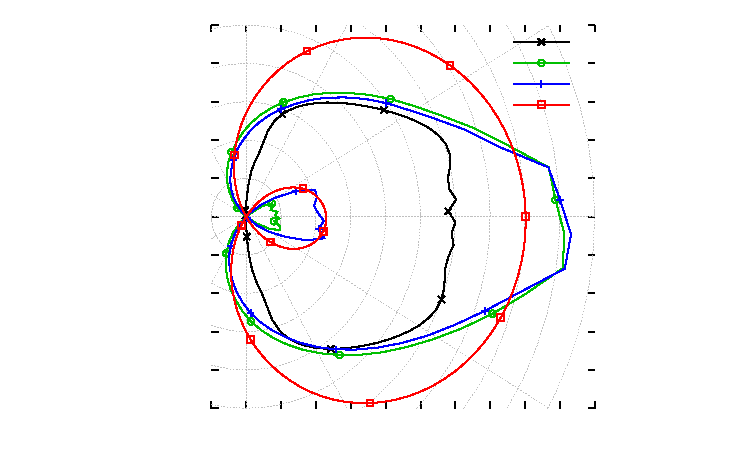
\includegraphics{/Users/seth/_thesis/figures/crashpipe2b/intens-x1-t1/intensity-x1-t1.pdf}}%
    \gplfronttext
  \end{picture}%
\endgroup

  \hspace{-.5in}
  \caption{Scalar flux with an isotropic boundary condition.}
  \label{fig:isotropic}
\end{figure}

\begin{figure}[htb!]
  \centering
  \hspace{-.5in}
  % GNUPLOT: LaTeX picture with Postscript
\begingroup
  \makeatletter
  \providecommand\color[2][]{%
    \GenericError{(gnuplot) \space\space\space\@spaces}{%
      Package color not loaded in conjunction with
      terminal option `colourtext'%
    }{See the gnuplot documentation for explanation.%
    }{Either use 'blacktext' in gnuplot or load the package
      color.sty in LaTeX.}%
    \renewcommand\color[2][]{}%
  }%
  \providecommand\includegraphics[2][]{%
    \GenericError{(gnuplot) \space\space\space\@spaces}{%
      Package graphicx or graphics not loaded%
    }{See the gnuplot documentation for explanation.%
    }{The gnuplot epslatex terminal needs graphicx.sty or graphics.sty.}%
    \renewcommand\includegraphics[2][]{}%
  }%
  \providecommand\rotatebox[2]{#2}%
  \@ifundefined{ifGPcolor}{%
    \newif\ifGPcolor
    \GPcolortrue
  }{}%
  \@ifundefined{ifGPblacktext}{%
    \newif\ifGPblacktext
    \GPblacktexttrue
  }{}%
  % define a \g@addto@macro without @ in the name:
  \let\gplgaddtomacro\g@addto@macro
  % define empty templates for all commands taking text:
  \gdef\gplbacktext{}%
  \gdef\gplfronttext{}%
  \makeatother
  \ifGPblacktext
    % no textcolor at all
    \def\colorrgb#1{}%
    \def\colorgray#1{}%
  \else
    % gray or color?
    \ifGPcolor
      \def\colorrgb#1{\color[rgb]{#1}}%
      \def\colorgray#1{\color[gray]{#1}}%
      \expandafter\def\csname LTw\endcsname{\color{white}}%
      \expandafter\def\csname LTb\endcsname{\color{black}}%
      \expandafter\def\csname LTa\endcsname{\color{black}}%
      \expandafter\def\csname LT0\endcsname{\color[rgb]{1,0,0}}%
      \expandafter\def\csname LT1\endcsname{\color[rgb]{0,1,0}}%
      \expandafter\def\csname LT2\endcsname{\color[rgb]{0,0,1}}%
      \expandafter\def\csname LT3\endcsname{\color[rgb]{1,0,1}}%
      \expandafter\def\csname LT4\endcsname{\color[rgb]{0,1,1}}%
      \expandafter\def\csname LT5\endcsname{\color[rgb]{1,1,0}}%
      \expandafter\def\csname LT6\endcsname{\color[rgb]{0,0,0}}%
      \expandafter\def\csname LT7\endcsname{\color[rgb]{1,0.3,0}}%
      \expandafter\def\csname LT8\endcsname{\color[rgb]{0.5,0.5,0.5}}%
    \else
      % gray
      \def\colorrgb#1{\color{black}}%
      \def\colorgray#1{\color[gray]{#1}}%
      \expandafter\def\csname LTw\endcsname{\color{white}}%
      \expandafter\def\csname LTb\endcsname{\color{black}}%
      \expandafter\def\csname LTa\endcsname{\color{black}}%
      \expandafter\def\csname LT0\endcsname{\color{black}}%
      \expandafter\def\csname LT1\endcsname{\color{black}}%
      \expandafter\def\csname LT2\endcsname{\color{black}}%
      \expandafter\def\csname LT3\endcsname{\color{black}}%
      \expandafter\def\csname LT4\endcsname{\color{black}}%
      \expandafter\def\csname LT5\endcsname{\color{black}}%
      \expandafter\def\csname LT6\endcsname{\color{black}}%
      \expandafter\def\csname LT7\endcsname{\color{black}}%
      \expandafter\def\csname LT8\endcsname{\color{black}}%
    \fi
  \fi
  \setlength{\unitlength}{0.0500bp}%
  \begin{picture}(7200.00,4320.00)%
    \gplgaddtomacro\gplbacktext{%
      \csname LTb\endcsname%
      \put(1910,400){\makebox(0,0)[r]{\strut{} 0.1}}%
      \put(1910,768){\makebox(0,0)[r]{\strut{} 0.08}}%
      \put(1910,1136){\makebox(0,0)[r]{\strut{} 0.06}}%
      \put(1910,1504){\makebox(0,0)[r]{\strut{} 0.04}}%
      \put(1910,1872){\makebox(0,0)[r]{\strut{} 0.02}}%
      \put(1910,2240){\makebox(0,0)[r]{\strut{} 0}}%
      \put(1910,2607){\makebox(0,0)[r]{\strut{} 0.02}}%
      \put(1910,2975){\makebox(0,0)[r]{\strut{} 0.04}}%
      \put(1910,3343){\makebox(0,0)[r]{\strut{} 0.06}}%
      \put(1910,3711){\makebox(0,0)[r]{\strut{} 0.08}}%
      \put(1910,4079){\makebox(0,0)[r]{\strut{} 0.1}}%
      \csname LTb\endcsname%
      \put(2030,200){\makebox(0,0){\strut{} 0.02}}%
      \csname LTb\endcsname%
      \put(2364,200){\makebox(0,0){\strut{} 0}}%
      \csname LTb\endcsname%
      \put(2699,200){\makebox(0,0){\strut{} 0.02}}%
      \csname LTb\endcsname%
      \put(3033,200){\makebox(0,0){\strut{} 0.04}}%
      \csname LTb\endcsname%
      \put(3368,200){\makebox(0,0){\strut{} 0.06}}%
      \csname LTb\endcsname%
      \put(3702,200){\makebox(0,0){\strut{} 0.08}}%
      \csname LTb\endcsname%
      \put(4037,200){\makebox(0,0){\strut{} 0.1}}%
      \csname LTb\endcsname%
      \put(4371,200){\makebox(0,0){\strut{} 0.12}}%
      \csname LTb\endcsname%
      \put(4706,200){\makebox(0,0){\strut{} 0.14}}%
      \csname LTb\endcsname%
      \put(5040,200){\makebox(0,0){\strut{} 0.16}}%
      \csname LTb\endcsname%
      \put(5375,200){\makebox(0,0){\strut{} 0.18}}%
      \csname LTb\endcsname%
      \put(5709,200){\makebox(0,0){\strut{} 0.2}}%
      \csname LTb\endcsname%
      \put(1330,2239){\rotatebox{-270}{\makebox(0,0){\strut{}x1 center $(1.01,3.5)$}}}%
    }%
    \gplgaddtomacro\gplfronttext{%
      \csname LTb\endcsname%
      \put(4806,3916){\makebox(0,0)[r]{\strut{}S$_{128}$}}%
      \csname LTb\endcsname%
      \put(4806,3716){\makebox(0,0)[r]{\strut{}FLAD$_{64}$}}%
      \csname LTb\endcsname%
      \put(4806,3516){\makebox(0,0)[r]{\strut{}AD$_{64}$}}%
      \csname LTb\endcsname%
      \put(4806,3316){\makebox(0,0)[r]{\strut{}FLD}}%
    }%
    \gplbacktext
    \put(0,0){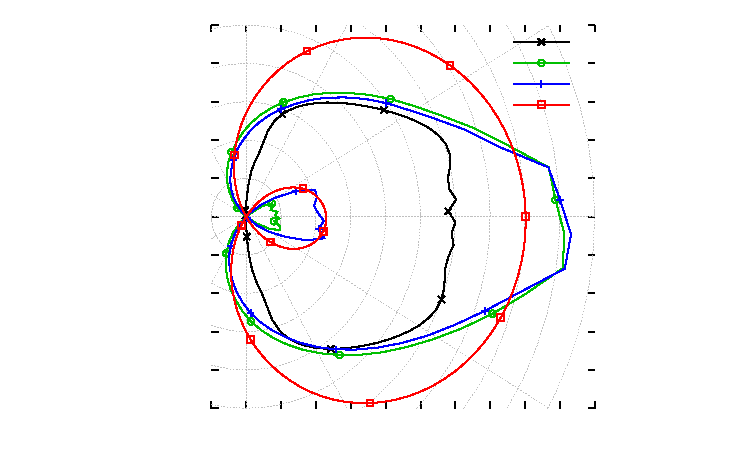
\includegraphics{/Users/seth/_thesis/figures/crashpipe2b/intens-x1-t1/intensity-x1-t1.pdf}}%
    \gplfronttext
  \end{picture}%
\endgroup

  \hspace{-.5in}
  \caption{Scalar flux with a normally incident boundary condition.}
  \label{fig:delta}
\end{figure}

\begin{figure}[htb!]
  \centering
  \hspace{-.5in}
  % GNUPLOT: LaTeX picture with Postscript
\begingroup
  \makeatletter
  \providecommand\color[2][]{%
    \GenericError{(gnuplot) \space\space\space\@spaces}{%
      Package color not loaded in conjunction with
      terminal option `colourtext'%
    }{See the gnuplot documentation for explanation.%
    }{Either use 'blacktext' in gnuplot or load the package
      color.sty in LaTeX.}%
    \renewcommand\color[2][]{}%
  }%
  \providecommand\includegraphics[2][]{%
    \GenericError{(gnuplot) \space\space\space\@spaces}{%
      Package graphicx or graphics not loaded%
    }{See the gnuplot documentation for explanation.%
    }{The gnuplot epslatex terminal needs graphicx.sty or graphics.sty.}%
    \renewcommand\includegraphics[2][]{}%
  }%
  \providecommand\rotatebox[2]{#2}%
  \@ifundefined{ifGPcolor}{%
    \newif\ifGPcolor
    \GPcolortrue
  }{}%
  \@ifundefined{ifGPblacktext}{%
    \newif\ifGPblacktext
    \GPblacktexttrue
  }{}%
  % define a \g@addto@macro without @ in the name:
  \let\gplgaddtomacro\g@addto@macro
  % define empty templates for all commands taking text:
  \gdef\gplbacktext{}%
  \gdef\gplfronttext{}%
  \makeatother
  \ifGPblacktext
    % no textcolor at all
    \def\colorrgb#1{}%
    \def\colorgray#1{}%
  \else
    % gray or color?
    \ifGPcolor
      \def\colorrgb#1{\color[rgb]{#1}}%
      \def\colorgray#1{\color[gray]{#1}}%
      \expandafter\def\csname LTw\endcsname{\color{white}}%
      \expandafter\def\csname LTb\endcsname{\color{black}}%
      \expandafter\def\csname LTa\endcsname{\color{black}}%
      \expandafter\def\csname LT0\endcsname{\color[rgb]{1,0,0}}%
      \expandafter\def\csname LT1\endcsname{\color[rgb]{0,1,0}}%
      \expandafter\def\csname LT2\endcsname{\color[rgb]{0,0,1}}%
      \expandafter\def\csname LT3\endcsname{\color[rgb]{1,0,1}}%
      \expandafter\def\csname LT4\endcsname{\color[rgb]{0,1,1}}%
      \expandafter\def\csname LT5\endcsname{\color[rgb]{1,1,0}}%
      \expandafter\def\csname LT6\endcsname{\color[rgb]{0,0,0}}%
      \expandafter\def\csname LT7\endcsname{\color[rgb]{1,0.3,0}}%
      \expandafter\def\csname LT8\endcsname{\color[rgb]{0.5,0.5,0.5}}%
    \else
      % gray
      \def\colorrgb#1{\color{black}}%
      \def\colorgray#1{\color[gray]{#1}}%
      \expandafter\def\csname LTw\endcsname{\color{white}}%
      \expandafter\def\csname LTb\endcsname{\color{black}}%
      \expandafter\def\csname LTa\endcsname{\color{black}}%
      \expandafter\def\csname LT0\endcsname{\color{black}}%
      \expandafter\def\csname LT1\endcsname{\color{black}}%
      \expandafter\def\csname LT2\endcsname{\color{black}}%
      \expandafter\def\csname LT3\endcsname{\color{black}}%
      \expandafter\def\csname LT4\endcsname{\color{black}}%
      \expandafter\def\csname LT5\endcsname{\color{black}}%
      \expandafter\def\csname LT6\endcsname{\color{black}}%
      \expandafter\def\csname LT7\endcsname{\color{black}}%
      \expandafter\def\csname LT8\endcsname{\color{black}}%
    \fi
  \fi
  \setlength{\unitlength}{0.0500bp}%
  \begin{picture}(7200.00,4320.00)%
    \gplgaddtomacro\gplbacktext{%
      \csname LTb\endcsname%
      \put(1910,400){\makebox(0,0)[r]{\strut{} 0.1}}%
      \put(1910,768){\makebox(0,0)[r]{\strut{} 0.08}}%
      \put(1910,1136){\makebox(0,0)[r]{\strut{} 0.06}}%
      \put(1910,1504){\makebox(0,0)[r]{\strut{} 0.04}}%
      \put(1910,1872){\makebox(0,0)[r]{\strut{} 0.02}}%
      \put(1910,2240){\makebox(0,0)[r]{\strut{} 0}}%
      \put(1910,2607){\makebox(0,0)[r]{\strut{} 0.02}}%
      \put(1910,2975){\makebox(0,0)[r]{\strut{} 0.04}}%
      \put(1910,3343){\makebox(0,0)[r]{\strut{} 0.06}}%
      \put(1910,3711){\makebox(0,0)[r]{\strut{} 0.08}}%
      \put(1910,4079){\makebox(0,0)[r]{\strut{} 0.1}}%
      \csname LTb\endcsname%
      \put(2030,200){\makebox(0,0){\strut{} 0.02}}%
      \csname LTb\endcsname%
      \put(2364,200){\makebox(0,0){\strut{} 0}}%
      \csname LTb\endcsname%
      \put(2699,200){\makebox(0,0){\strut{} 0.02}}%
      \csname LTb\endcsname%
      \put(3033,200){\makebox(0,0){\strut{} 0.04}}%
      \csname LTb\endcsname%
      \put(3368,200){\makebox(0,0){\strut{} 0.06}}%
      \csname LTb\endcsname%
      \put(3702,200){\makebox(0,0){\strut{} 0.08}}%
      \csname LTb\endcsname%
      \put(4037,200){\makebox(0,0){\strut{} 0.1}}%
      \csname LTb\endcsname%
      \put(4371,200){\makebox(0,0){\strut{} 0.12}}%
      \csname LTb\endcsname%
      \put(4706,200){\makebox(0,0){\strut{} 0.14}}%
      \csname LTb\endcsname%
      \put(5040,200){\makebox(0,0){\strut{} 0.16}}%
      \csname LTb\endcsname%
      \put(5375,200){\makebox(0,0){\strut{} 0.18}}%
      \csname LTb\endcsname%
      \put(5709,200){\makebox(0,0){\strut{} 0.2}}%
      \csname LTb\endcsname%
      \put(1330,2239){\rotatebox{-270}{\makebox(0,0){\strut{}x1 center $(1.01,3.5)$}}}%
    }%
    \gplgaddtomacro\gplfronttext{%
      \csname LTb\endcsname%
      \put(4806,3916){\makebox(0,0)[r]{\strut{}S$_{128}$}}%
      \csname LTb\endcsname%
      \put(4806,3716){\makebox(0,0)[r]{\strut{}FLAD$_{64}$}}%
      \csname LTb\endcsname%
      \put(4806,3516){\makebox(0,0)[r]{\strut{}AD$_{64}$}}%
      \csname LTb\endcsname%
      \put(4806,3316){\makebox(0,0)[r]{\strut{}FLD}}%
    }%
    \gplbacktext
    \put(0,0){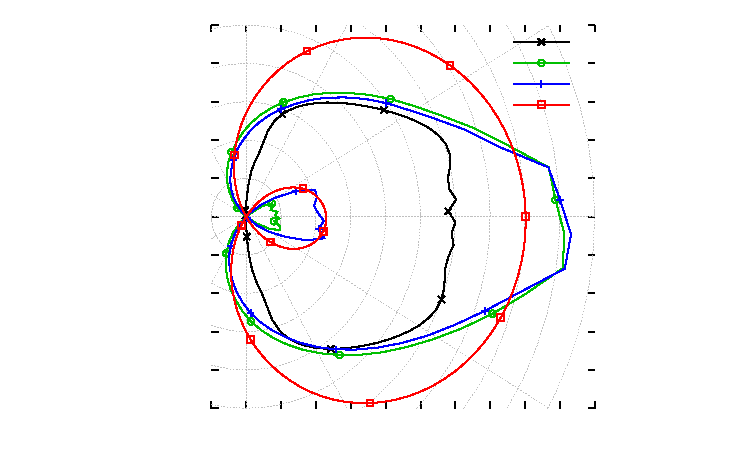
\includegraphics{/Users/seth/_thesis/figures/crashpipe2b/intens-x1-t1/intensity-x1-t1.pdf}}%
    \gplfronttext
  \end{picture}%
\endgroup

  \hspace{-.5in}
  \caption{Scalar flux with a grazing boundary condition.}
  \label{fig:grazing}
\end{figure}

%%%%%%%%%%%%%%%%%%%%%%%%%%%%%%%%%%%%%%%%%%%%%%%%%%%%%%%%%%%%%%%%%%%%%%%%%%%%%%%%
\section{Conclusions}
We successfully derived and tested both Marshak and variational boundary
conditions for diffusion in flatland geometry. Both boundary conditions are
markedly different from the standard diffusion boundary conditions.

The Marshak boundary, which uses $\pi \int_{\vec{\Omega}\vd \vec{n} < 0 }
\abs{\vec{\Omega}\vd \vec{n}} \psi^b \ud\Omega$, gives an extrapolation
distance for flatland of about $0.7854$.
The more accurate boundary condition given in Eq.~\eqref{eq:flatVarBc} uses 
$\int_{\vec{\Omega}\vd\vec{n} < 0} \left[ \frac{\pi}{2}
\abs{\vec{\Omega}\vd\vec{n}} + 2 (\vec{\Omega}\vd\vec{n})^2 \right]
\psi^b(\vec{x}, \vec{\Omega}) \ud\Omega$ with the extrapolation distance of
about $0.8171$.

%%%%%%%%%%%%%%%%%%%%%%%%%%%%%%%%%%%%%%%%%%%%%%%%%%%%%%%%%%%%%%%%%%%%%%%%%%%%%%%%
\bibliographystyle{ans}
\bibliography{../SRJall}
\end{document}
